%
% File: chap02.tex
% Author: Your Name
% Description: Methodology
%
\let\textcircled=\pgftextcircled
\chapter{Theoretical Background}
\label{chap:intro}

\section{Green Bond Market}
\initial{F}inancial markets play a critical role in the transition to a low-carbon economy by mobilizing and allocating investments in green projects \citep[p. 3]{oecd2021}. One way to increase these investments is to develop and deploy a new set of financial instruments. The first institutions to express a desire and interest in sustainable investments were Scandinavian pension funds. The International Bank for Reconstruction and Development (IBRD), managed by the World Bank, seized on this desire and partnered with these institutional investors in 2008 to develop and deploy a new type of debt financing instrument - the green bond \citep[p. 24]{worldbank2015}. Unlike conventional bonds, green bonds are issued to raise capital specifically to support environmental or climate projects [p. 23]. For this purpose, the first green bond was issued in November 2008 for an amount of approximately USD 440 million (SEK 3.35 billion). This simple fixed-income product helped the World Bank to further raise awareness of climate change in the financial community and provide investors with an investment vehicle to take action [p. 24]. With the rapid growth of the market, the following unanswered questions emerged: Which bond-financed projects qualify for a green label? Who is responsible for the due diligence requirements and process? As a result, market participants needed a framework to clarify the vague definitions and processes pertaining to green bonds, reducing asymmetric information between issuers and investors. The procedure for a green flag can therefore also be seen as another textbook example of \cite{akerlof1970market}'s market of lemons. In early 2014, a group of banks initiated the development of the Green Bond Principles (GBP), based on the practice and experience of pioneers among multilateral development banks. The GBP act as voluntary guidelines to the issuance of green bonds and are intended to promote transparency, disclosure and integrity in the development of the green bond market [p. 30]:
 
 
\vspace{.3cm}

\textit{
"The GBP suggests a process for designating, disclosing, managing, and reporting on the proceeds of the bond. They are designed to provide issueres with guidance on the key components involved in launcing a green bond, including providing information to aids investors in evaluating the environmental impact of their green bond investments \citep[p. 30]{worldbank2015}."}

\vspace{.3cm}
Therefore, an important part of the framework is to address the potential information asymmetries between issuers and investors. Accordingly, in addition to issuer disclosures addressed by the framework, market participants rely on the second opinions and comments from academics, investment advisors, auditors, technical experts, media, and non-governmental organizations (NGOs) such as CICERO, the Climate Bonds Initiative, Det Norske Veritas (DNV), Norway, Oekom, Sustainalytics, and Vigeo, among others, to ensure increased transparency \citep[p. 31]{worldbank2015}. 
The GBP defines the term "green bond," as follows \citep[p. 3]{international2022green}:
\vspace{.3cm}

\textit{
"Green bonds are any type of bond instrument where the proceeds or an equivalent amount will be exclusively applied to finance or re-finance, in part or in full, new and/or existing eligible green projects and which are aligned with the four core components of the GBP."} 
\vspace{.3cm}

These four core components are the following [p. 4]:

\begin{enumerate}
    \item \textit{Use of Proceeds};
    \item \textit{Process for Project Evaluation and Selection};
    \item \textit{Management of Proceeds};
    \item \textit{Reporting}.
\end{enumerate}

According to the GBP, a (non-exhaustive) list of categories recognized as potentially eligible projects are the following [pp. 4--5]:  

\begin{enumerate}
    \item \textit{Renewable} energy (including production, transmission, applicances and products);
    \item \textit{Energy efficiency} (such as in new and refurbished buildings, energy storage, district heating, smart grids, appliances and products);
    \item \textit{Pollution prevention and control} (including reduction of air emissions, greenhouse gas control, soil remediation, waste prevention, waste reduction, waste recycling and energy/ emission-efficient waste to energy);
    \item \textit{Environmentally sustainable management of living natural resources and land use} (including environmentally sustainable agriculture; environmentally sustainable animal husbandry; climate smart farm inputs such as biological crop protection or drip-irrigation; environmentally sustainable fishery and aquaculture; environmentally sustainable forestry, including afforestation or reforestation, and preservation or restoration of natural landscapes);
    \item \textit{Terrestrial and aquatic biodiversity conservation} (including the protection of coastal, marine and watershed environments);
    \item \textit{Clean transportation} (such as electric, hybrid, public, rail, non-motorised, multi-modal transportation, infrastructure for clean energy vehicles and reduction of harmful emissions);
    \item \textit{Sustainable water and wastewater management} (including sustainable infrastructure for clean and/or drinking water, wastewater treatment, sustainable urban drainage systems and river training and other forms of flooding mitigation);
    \item \textit{Climate change adaptation} (including efforts to make infrastructure more resilient to impacts of climate change, as well as information support systems, such as climate observation and early warning systems);
    \item \textit{Circular economy adapted products, production technologies and processes} (such as the design and introduction of reusable, recyclable and refurbished materials, components and products; circular tools and services); and/or certified eco-efficient products;
    \item \textit{Green buildings} that meet regional, national or internationally recognised standards or certifications for environmental performance.
\end{enumerate}

With these theoretical considerations about green bonds in mind, we can now move on to some key statistics and figures that illustrate the evolution and characteristics of the green bond market. First, Figure \ref{evo1} illustrates the development of the amounts issued by currency or bundled currency area per year according to the Eikon Refinitiv green bond universe database. The first observation that can be made is that the green bond market grows exponentially every two years until 2021, when the amount issued reaches a record USD 600 billion. Next, the largest two markets by currency are Euro and U.S. Dollar. In addition, the Chinese yuan quickly gained a place in the top 3 after Shanghai Pudong Development Bank issued its first green bond in 2016 \citep[p. 1]{wang2020market}.

Second, Figure \ref{evo2} visualizes the same histogram but clustered by the type of issuer. We categorized the issuers in four broad categories:

\begin{enumerate}
    \item \textit{Agency}: Bonds issuer by U.S. government agencies including publicly owned U.S. government-sponsored enterprises (GSEs);
    \item \textit{Corporate}: Bonds issued by firms;
    \item \textit{Govt/Treasuy/Central Bank}: Bonds issued by the Government, Treasury or Central Bank;
    \item \textit{Other Gov/Supra}: Bonds issued by Supranational Entities.
\end{enumerate}

It can be observed that corporations are the largest issuer of green bonds, followed by the public sector, which is not consistent with the overall global debt security market, where the public and private sectors are more balanced. In addition, the amount outstanding in the overall global debt security market is over \$120 trillion in 2022. Thus, the proportion of the green bond market is relatively small at $\approx0.25\%$.\footnote{For a detailed overview visit \url{https://www.bis.org/statistics/about_securities_stats.htm}}

Finally, Figure \ref{map} visualizes a global heat-map of the amount of green bonds issued in each country. The U.S. ranks first, followed by European countries and China. It is also noticeable that almost no African country, Eastern European country or Western Asian country has issued a green bond yet.

\begin{center}
\begin{figure}[h!]
    \centering
    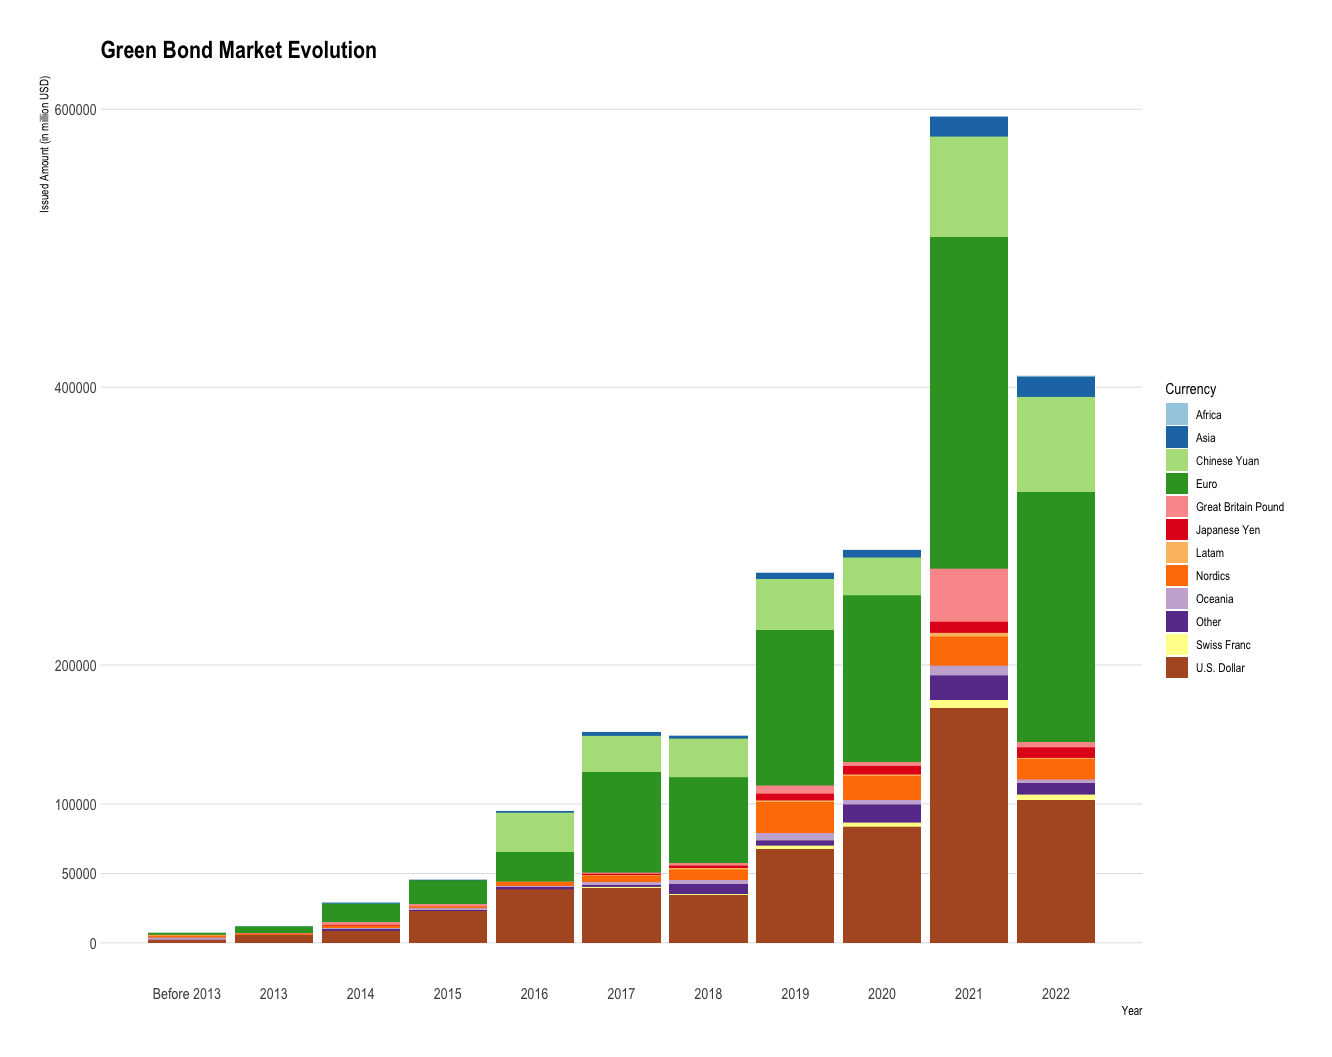
\includegraphics[scale=0.35]{chinchilab-template/chapters/chapter02/Green Bond Market Evolution.png}
    \caption{Green Bond Market Evolution by Currency / Currency Basket (own illustration).}
    \caption*{\scriptsize{\textbf{Source}: Eikon Refinitiv Green Bond Universe. \textbf{Green Bond types included}: Self-labeled, CBI certified, CBI aligned. \textbf{Africa}: Moroccan Dirham, Namibian Dollar, Nigerian Naira, South African Rand. \textbf{Asia}: Bangladeshi Taka, Hong Kong Dollar, Indian Rupee, Indonesian Rupiah, Macanese Pataca, Malaysian Ringgit, Philippine Peso, Singapore Dollar, Sri Lankan Rupee, South Korean Won, Taiwan Dollar, Thai Baht, Vietnamese Dong. \textbf{Latam}: Argentine Peso, Argentine Unidades de Valor Adquisitivo, Brazilian Real, Chilean Peso, Chilean Unidad de Fomento, Colombian Peso, Peruvian Sol. \textbf{Nordics}: Danish Krone, Icelandic Krona, Norwegian Krone, Swedish Krona. \textbf{Oceania}: Australian Dollar, Fijian Dollar, New Zealand Dollar. \textbf{Other}: Canadian Dollar, Czech Koruna, Deutsche Mark, Hungarian Forint, Kazakhstani Tenge, Polish Zloty, Romanian Leu, Russian Ruble, Turkish Lira, Ukrainian Hryvnia.}}
    \label{evo1}
\end{figure}

\begin{figure}[h!]
    \centering
    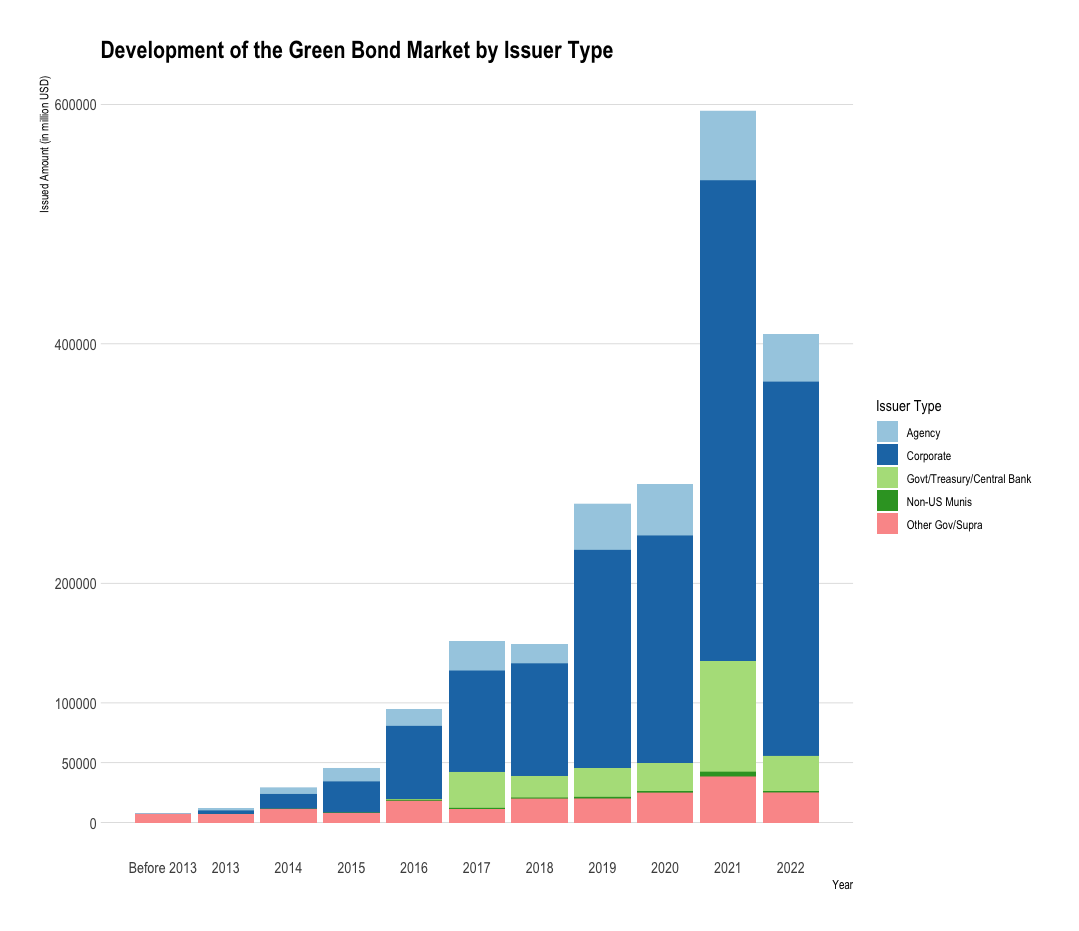
\includegraphics[scale=0.42]{chinchilab-template/chapters/chapter02/Issuer Type.png}
    \caption{Green Bond Market Evolution by Type of Issuer (own illustration).}
    \caption*{\scriptsize{ \textbf{Source}: Eikon Refinitiv Green Bond Universe.}}
    \label{evo2}
\end{figure}
\end{center}


\begin{sidewaysfigure}[htbp!]
    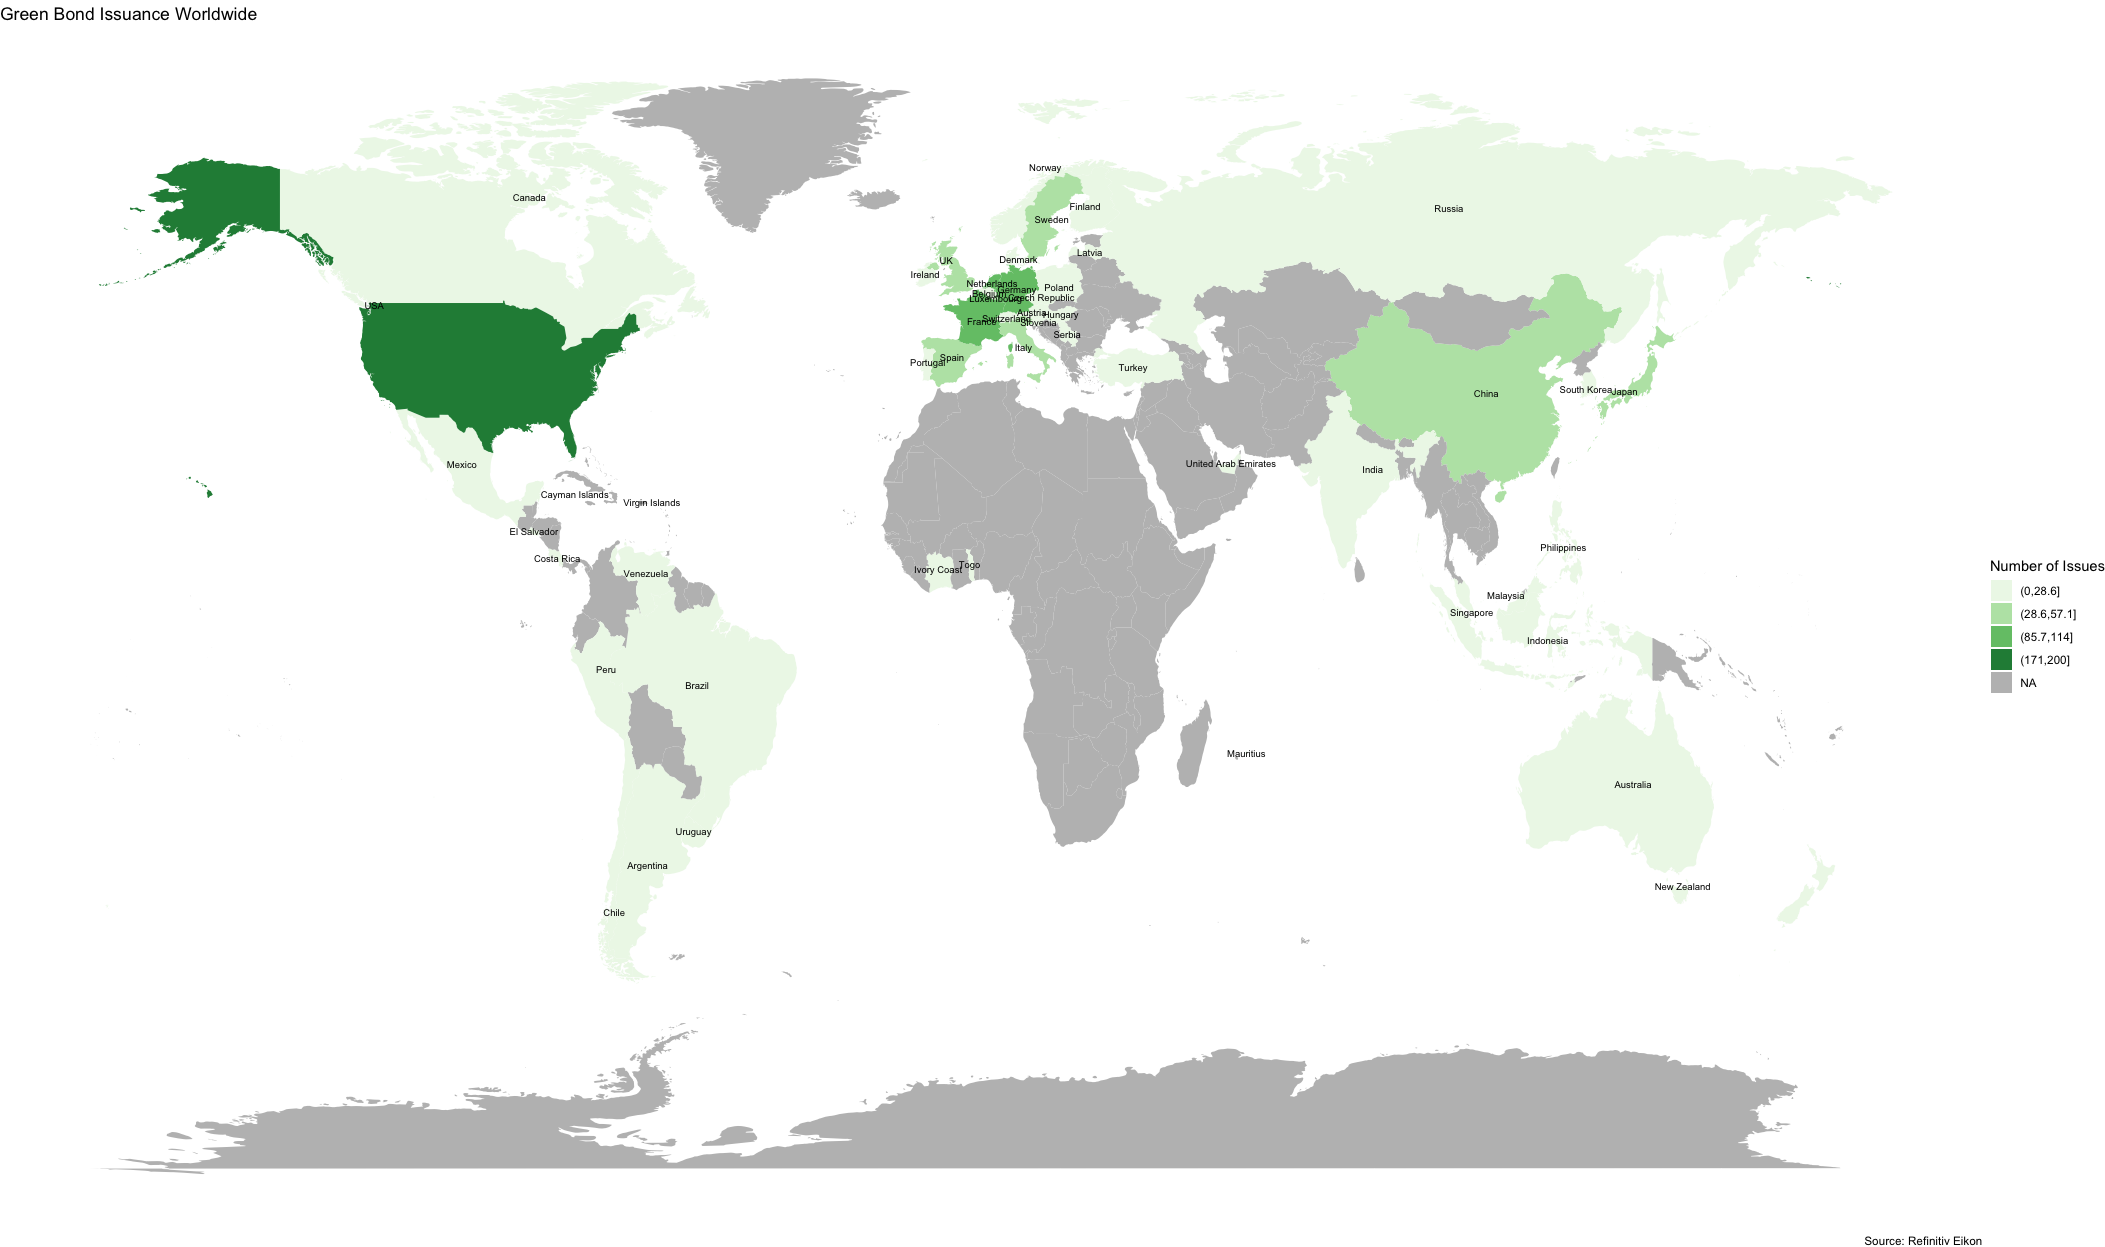
\includegraphics[width=\textwidth]{chinchilab-template/chapters/chapter02/Map.png}
    \caption{Global Heatmap of Amount of Green Bonds Issued by Country (own illustration).}
    \label{map}
\end{sidewaysfigure}

 
\section{Greenium}

In 2016, first anecdotal evidence\footnote{See e.g. \citet{barclays}.} emerged that, at least in some markets, green bonds were fetching better prices than regular "vanilla" bonds. This phenomenon has been coined "greenium". The implication is that green bonds have a higher price and lower yields due to the inverse relationship between bond prices and yields. For the issuer, i.e. the debtor of the bond, this is advantageous because it means a lower cost of capital. However, for the investor who buys the green bond at a higher price, this means foregoing a lower price for conventional bonds, assuming that there is no difference between green and conventional bonds except for the green flag \citep[p. 19]{cbi2016}. Taking into account standard finance theory, where only the trade-off between risk and return plays a role in an investor's decision-making process, an investor's willingness to pay a higher price for a green bond would be irrational. In addition, it can be observed in the bond market that vanilla bonds are usually somewhat cheaper than seasoned bonds of the same issuer. This so-called new issue premium is sponsored by the issuer to attract investment \citep[p. 10]{cbi2017}. 

A capital market essentially comprises both primary and secondary markets. However, this study is exclusively concerned with the primary market. Therefore, the next paragraph summarizes the literature that has emerged since 2016 on whether the greenium exists in the primary market for green bonds and, if so, what the determinants are.

\section{Literature Review}

The first study to empirically test the anecdotal evidence of a greenium was conducted in 2016 by the Climate Bonds Initiative (CBI), an international organisation that works to mobilize global capital for climate action. In the primary market analysis, their sample consisted of 10 U.S. Dollar green bonds and 4 Euro green bonds issued between January 2016 and March 2017. They analyzed the yield curve of these 7 corporate green bond issuers individually and their results showed that (1) 6 bonds were priced within their own yield curve, indicating that there exists a greenium (no issuance premium), (2) 4 bonds were priced on their own yield curve, indicating the absence of a new issue premium, and (3) 4 bonds were priced outside their own yield curve suggesting the presence of a new issue premium. In summary, the findings show no difference between the issue prices of green and brown bonds \citep[p. 10]{cbi2017}.

In a study conducted by the Bank for International Settlements, \citet{ehlers2017green} compared credit spreads\footnote{Spread of yield at issuance - yield curve of U.S. Treasury security.} on the issuance of a cross-section of 21 green bonds issued between 2014 and 2017 with credit spreads on the issuance of plain vanilla bonds of the same issuers at the nearest possible issue date. More specifically, the sample was limited to pari-passu bonds with a maturity of at least two years, a par value of \$10 million and denomination in U.S. dollars or euros. The results show that, compared to conventional bond spreads, green bond spreads are, on average, 18 basis points lower. In addition, green bonds with lower issuer ratings carry wider spreads. The authors conclude that the results are consistent with the fact that demand for green bonds is high relative to supply and that lower issuer ratings imply higher credit risk. However, the results should be taken with a grain of salt, as the more detailed assessment shows some variability in the results, with a standard deviation of 27 basis points \citep[pp. 97--98]{ehlers2017green}.

Although the following paper analyzes the secondary market, it is crucial for further research from a methodological point of view. To our knowledge, \citet{zerbib2017green} is the first scientific paper to investigate the existence of greenium. He applies a matching method, also termed the model-free approach or direct approach, which is commonly used in later studies. The matching method involves finding a pair of instruments with the same characteristics, except for the characteristic of interest, in order to quantify its effects. The advantage of this method over the standard toolkit of regressions with an appropriate specification is that we can easily encounter problems, for instance, when there are too many covariates, which can result in collinearity, lack of data, and lack of robustness. Such a situation is particularly aggravated in a setting with a small number of observations, which is often the case in green bond analysis [p. 10]. In Zerbib's matching method, a green bond is paired with a synthetic conventional bond that has exactly the same characteristics (i.e. same issuer, currency, rating, bond structure, seniority, collateral and same coupon type). Since exact maturity matching is not possible, Zerbib allows for the maturity of the conventional bonds to be two years shorter or two years longer than the green bond. Based on this universe of matching bonds, he selects the pair with the closest maturity. In addition, only conventional bonds whose issue volume is at least one quarter that of a green bond are eligible, and only conventional bonds whose issue date is no more than six years before or after the issue date of the green bond are considered. After this matching procedure, the maturity bias between the green bond and the synthetic bond is eliminated. A synthetic bond is actually a synthesis of two conventional bonds, which is why it is often referred to as a bond triplet. To eliminate the maturity bias, Zerbib uses conventional bond yields to linearly interpolate or extrapolate them at the green bond's maturity date to obtain a synthetic conventional bond yield that mimics the green bond's characteristics. If the term to maturity of the green bond is shorter or longer than the term of both conventional bonds, extrapolation is used. In all other cases, interpolation is used [pp. 12ff.].

\citet{partridge2018green}'s study builds on the idea of yield curve analysis from \citet{cbi2017}. They conducted the first study in this field to quantify the greenium in the primary municipal bond market [p. 3]. Based on 50 series of municipal bonds issued between June 2013 and January 2018, green and conventional bond pairs were matched against one another based on the same issuer, use of proceeds, issue date, maturity date, and coupon, resulting in a total of 521 pairs [p. 5]. To obtain the yield curves, the authors utilized the Svensson technique [p. 8]. Their results show that between 2014 and 2016, vanilla bonds were sold at a premium, while green bonds were sold at a discount. However, in 2017, the situation reversed and green bonds were sold at a 1 basis point premium [p. 12]. In terms of spreads, the overall weighted average greenium was 4 basis points overall, with an upward trend [p. 16].

The following study is the first and one of the few to embed its analysis in a theoretical framework. \citet{baker2018financing} derive an asset pricing framework to understand how non-pecuniary objectives affect prices and portfolio choice.\footnote{The predictions derived are similar to \citet{fama2007disagreement} who model the "taste" effects on asset prices.} The model's prediction is twofold: (1) Securities with positive environmental scores have lower expected returns [p. 1] and (2) have more concentrated ownership, particularly for those with low market values and low risk [p. 28]. For their empirical analysis, the authors examine the U.S. corporate and municipal green bond markets. The corporate bonds are restricted to a sample of bonds issued between 2014 and 2016, while the municipal bonds sample includes bonds issued between 2010 and 2016 [p. 6]. \citet{baker2018financing} employ OLS regressions with fixed effects such as month, issuer, and yield curve. The results show the same overall pattern in all specifications: green bonds are sold at a moderate premium. Another result worth noting is that CBI-certified green bonds commanded a higher premium than non-certified CBI green bonds [pp. 21ff.]. Moreover, the analysis supports the second prediction of their framework that green bond ownership is more concentrated. This applies in particular to bonds with a low nominal value and low risk (high rating) [p. 32].

\citet{gianfrate2019green} contribute to the literature by adopting a propensity score matching (PSM) methodology to quantify the average treatment effect on the treated (ATT). The sample consists of bonds issued between January 2007 and December 2017. Only fixed coupon bonds, euro-denominated bonds with an issuance volume of at least EUR 200 million, and all bonds with a rating above BBB- were eligible. The final sample consists of 121 green bonds. The PSM method allows the estimation of the counterfactual condition, i.e., the unobservable condition that a green bond is not green. To obtain the most accurate estimate, a control group (conventional bonds) is required that is identical in all respects to the treated group (green bonds) except for the treatment attribute. Since such a situation is not achievable, one would focus on the control group, that is as similar as possible to the treated group. The methodological procedure is as follows: (1) estimate the propensity score by predicting the probability that a bond is green (using either a Logit or Probit function) and (2) match treated units and control units based on the propensity score by using the nearest neighbors matching (NN) algorithm. Finally, calculate the average treatment effect of the treated (ATT).\footnote{ATT$=\mathrm{E}\left[Y^1-Y^0 \mid D=1\right]$ = $\mathrm{E}\left[Y^1 \mid D=1\right]-\mathrm{E}\left[Y^0 \mid D=1\right]$.} The results show a highly significant (1\% level) estimate in all comparison groups, ranging from -14.8 to -19.4 basis points. This suggests that, on average, green bonds offer investors a lower return than their conventional counterparts. Moreover, if the issuer is a corporation (operating primarily in the utilities and energy sectors), the average advantage is -21 basis points, while it is lower at -15 basis points for non-corporation issuers [pp. 128ff.].

The next paper is from \citet{larcker2020s}, who examine the U.S. municipal bond market from June 2013 to July 2018, very similar to \citet{partridge2018green}. However, \citet{larcker2020s} use a simple matching procedure in which they select (non-callable) bonds that were issued by the same issuer on the same day that have the same rating, coupon, and a maximum maturity difference of one year. For their final sample of 640 matched pairs, they calculate the average treatment effect (ATE).\footnote{ATE = $\hat{\tau}=\frac{1}{N}\sum_{i=1}^{N}(Y_i^{G}-Y_i^{NG})$} [pp. 7ff.] Using kernel density estimates of differences, paired t-tests, and Wilcoxon tests, their results show a statistically significant difference of about 0.4 basis points of yield difference, suggesting that green bonds are sold at a discount. However, the magnitude is economically insignificant and the results seem to be driven by outliers. Therefore, the authors conclude that the yield differential is exactly zero, which is in contrast to the results of \citet{partridge2018green} [pp. 10ff.].

\citet{tang2020shareholders} construct the most comprehensive international green bond dataset for the period June 2007 to July 2017, using an OLS regression with fixed effects by month, country, or issuer. The specification with country fixed effects as the sole factor yielded a significant greenium at the 5\% level. Issuer and month fixed effects were not statistically significant [p. 5; p. 11].

The following two paragraphs present studies that shed light on the presence of a greenium in the Chinese bond market. First, \citet{wang2020benefits} use a dataset of all green corporate bonds issued in mainland China from 2016 to 2020 Q2, which corresponds to 324 green bonds [p. 3]. Using the strict matching approach of \citet{larcker2020s} and the paired t-test as well as the Wilcoxon test, the authors find no difference in mean and median returns between green and conventional bonds [pp. 5f.]. Second, \citet{sheng2021financing} use a sample of all bonds issued on the Shanghai and Shenzhen stock exchanges and the interbank bond market from 2016 to 2018. They use propensity score matching with nearest neighbor matching to estimate the average treatment effects for the green bond (ATT). Depending on the specification, the ATT ranges from -0.37 to -0.22, but is highly significant at the 1\% threshold in all cases. As for the average difference between the issue yield of green and conventional bonds, the results show that it is -7.8 basis points for the whole sample. However, this result is due to the high mean value of the financial issuers, which amounts to -22.2 basis points. In addition, green bonds issued by state-owned enterprises (SOEs) have on average a higher greenium than non-SOEs [pp. 2644ff.]. 

\citet{agliardi2021corporate} provide the literature with a theoretical model of optimal portfolio allocation that can capture both a negative and a positive premium. The numerical simulation results are as follows: (1) the greenium becomes narrower when interest rates are lower, (2) uncertainty about the effectiveness of the green investment is negatively related to the greenium, (3) more effective technology increases the greenium, (4) volatile asset prices positively affect the greenium, (5) tax rates and greenium go in the same direction, and (6) the greenium is larger when the introduction of the green project directly benefits the core business, otherwise the greenium may even reverse its sign [pp. 271--272].

Correspondingly, \citet{kapraun2021credibly} develop a theoretical model, but in a microeconomic way. According to this model, households prefer green bonds with environmental impacts and are willing to pay a higher price for them than for bonds without environmental impacts. Moreover, households are willing to pay a higher price for green bonds issued by companies with a lower reputation for sustainability than for green bonds issued by companies with high environmental standards [p. 15]. To test the predictions, the authors collect a large green bond dataset of 2099 green bonds issued between January 2009 and February 2021 [p. 17]. As a first step, the study runs a fixed-effects OLS regression that yields an average of 12.8 basis points lower return for green bonds than for conventional bonds. However, when controlling for creditworthiness, this effect disappears. When the green bond is certified, there is a significant greenium of 16 basis points. Interestingly, 90\% of euro-denominated green bonds and 80\% of large green bonds are certified. Consequently, these specifications yield significant greeniums. Finally, green bonds issued by governments and supranational organizations command high premiums of about 18.5 basis points, while corporate bonds trade at significant discounts of about 6 basis points. Thus, the credibility of green projects seems to be an important factor explaining the presence of greenium [pp. 24ff.]. In a second step, \citet{kapraun2021credibly} use the matching method of \citet{zerbib2017green}, but with stricter bounds on maturity and issue size [pp. 17--18]. The yield difference of the 658 matched bonds shows that the issue yield of green bonds is on average 7.2 basis points lower than that of conventional bonds. Nevertheless, the authors conclude that their results show insignificant greenium on average [p. 29].

\citet{loffler2021drivers} also use a large dataset of green bonds issued between 2007 and October 2019 [p. 6]. Similar to \citet{gianfrate2019green}, they use a PSM method. As an extension, they also use Coarsened Exact Matching (CEM), which is arguably a better approach than PSM because it reduces model dependence as well as covariate imbalances between treated and controls [pp. 10f.]. Their analysis shows that green bond ask yields in the non-matching sample are 15 basis points lower than their counterparts. In the matched samples, the range of ask yields amount to 16-24 basis points [p. 14]. 

A very recent study that develops a theoretical model to explain greenium is the working paper by \citet{daubanes2021firms}. The authors derive a signaling model that captures the rationale behind managers' incentives to engage in CO2-reducing projects through certified green bonds [p. 6]. In a nutshell, their model derives an equilibrium condition in which the stock market reaction to a company's green bond issuance is positive. Therefore, managers constrain green bond issuance such that the stock market response remains positive. Moreover, this effect is amplified by carbon prices [p. 16ff.]. This is explained by the fact that green bonds are complementary to carbon prices. However, the authors conclude that this effect is probably due to a short-lived financial interest [p. 33].

The next study is again an empirical study covering green bonds issued globally between 2007 and 2018. \citet{fatica2021pricing} identified a total of 1397 green bonds for which they used the OLS fixed effects econometric strategy, which is very similar to \citet{baker2018financing} [pp. 5--6]. They arrive at the following results: Compared to ordinary bonds, only green bonds issued by supranational institutions and non-financial corporations sell at a premium. For instance, the premium for the former amounts to 80 basis points (1\% level), while for the latter it is 20 basis points (5\% level). For financial corporations, the difference in yield is not statistically significant. Moreover, the greenium for self-labeled green bonds is on average lower compared to externally reviewed bonds. The yield differential for one-time green bond issuers is also lower than for repeat issuers [pp. 6ff.].

Last but not least, \citet{caramichael2022green} also employ a fixed effects OLS regression on a dataset of 1169 green bonds issued between 2014 and 2021 [p. 3]. The following restrictions apply: Only fixed- or zero-coupon bonds issued in euros or U.S. dollars by private or state-owned companies with a notional value of at least USD 500 million are eligible [p. 8].
Their analysis shows a greenium of 8 basis points [p. 12]. Moreover, green bonds that are oversubscribed fetch a higher greenium. Specifically, a 1\% increase in oversubscription leads to a 0.058 basis point increase in the greenium. This idea that increased demand drives the greenium is also confirmed by controlling for the inclusion in a green bond index [pp. 17--18]. The authors conclude with the following finding: \textit{"While U.S. dollar- and euro-denominated green bonds capture comparable greeniums, we find that the greenium is allocated primarily to local euro and foreign U.S. dollar issuers. While green bond governance and external review appear to matter for the greenium, the credibility of the underlying projects does not have a significant impact. Instead, the greenium is unevenly distributed to large, investment-grade issuers, primarily within the banking sector and developed economies [p. 24]." }